\documentclass[12pt]{article}
\usepackage{graphicx}
\usepackage{subcaption}
\usepackage{float}
\usepackage{hyperref}

\title{EE236: Experiment 9\\
Temperature Dependence of Solar Cell Characteristics}

\author{Aaron John Sabu, 170070050}

\begin{document}
\maketitle

\section{Aim of the experiment}

The experiment aims to realise the variation of the I-V Characteristics of a solar cell as temperature is varied. Moreover the experiment deals with the variation of different parameters of a solar cell, such as ideality factor, fill factor, open-circuit voltage and short-circuit current, as the temperature of the solar cell is varied.

\section{Methods}

The experiment was performed using a temperature controlled oven and a temperature controller. This box comprised of a solar cell and an LED bank. moreover, it also contained a heating element which heated an aluminium slab on which the solar cell was placed. THe temperature of the solar cell was measured using an IC LM35. The temperature controller determined when to start and stop heating based on the output of LM35.\\
The voltmeter and ammeters were provided via the two portable Digital Multimeters and the provided one as well. As a common method for all three steps, the LEDs in the box were lighted using a voltage supply which was connected to the ammeter.

\subsection{Part 1}

The voltage source was connected to a 100 \(\Omega\) resistor which in turn was connected to the ammeter. The ammeter was connected to the n-terminal of the solar cell, whereas the p-terminal was connected to ground and the voltage across the solar cell was measured using a voltmeter.


\begin{figure}[H]
	\centering
	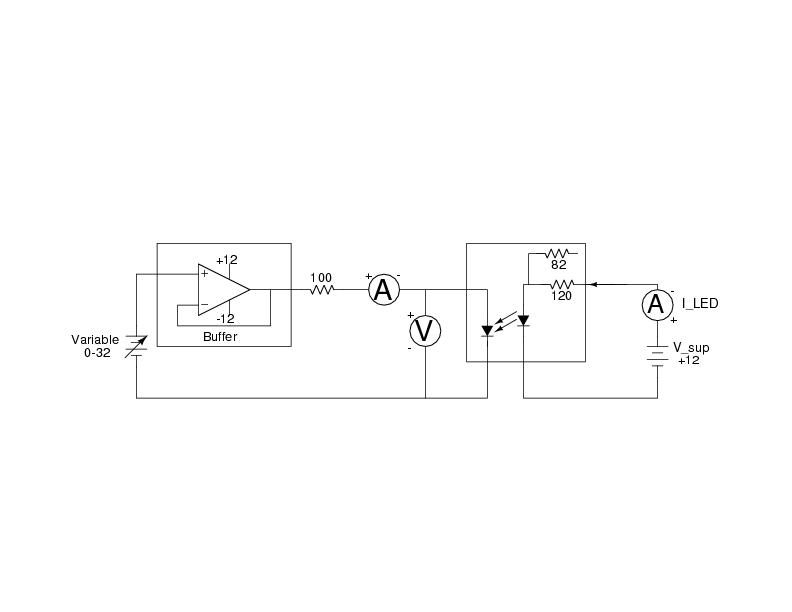
\includegraphics[width = \linewidth, trim = {2cm 2cm 0 2cm}, clip]{Part1_CD.png}
	\caption{Part 1 Circuit Diagram}
\end{figure}

\subsection{Part 2}

Two potentiometers, one of 500\(\Omega\) and one of 100\(\Omega\) were used in series. The one of higher resistance was used for coarse variation and the other one for fine variation. These were in turn connected to an ammeter. The ammeter and the voltmeter served the same purpose as in part 1.

\begin{figure}[H]
	\centering
	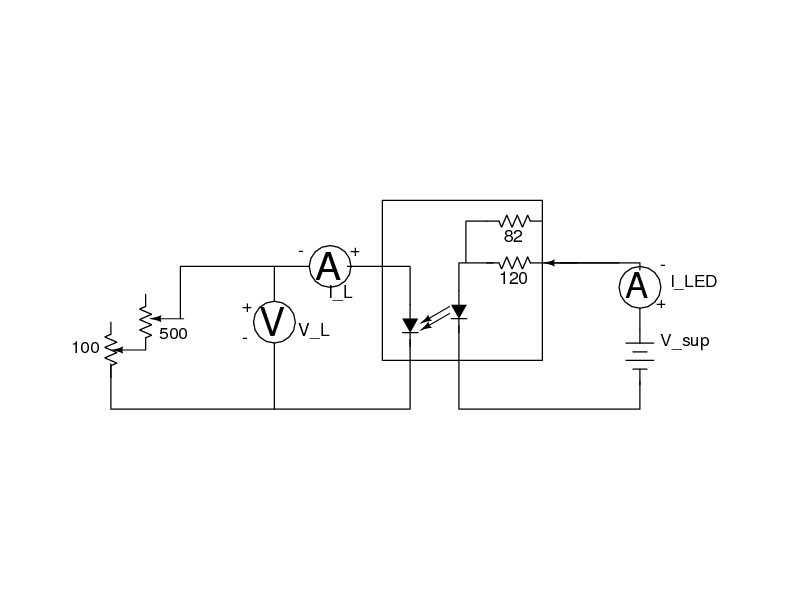
\includegraphics[width = \linewidth, trim = {0 2cm 1cm 2.5cm}, clip]{Part2_CD.png}
	\caption{Part 2 Circuit Diagram}
\end{figure}

\section{Observations}

The experiment was conducted at five different temperatures, \(35^{\circ}C\), \(45^{\circ}C\), \(55^{\circ}C\), \(65^{\circ}C\) and \(75^{\circ}C\). Here are the results we obtained:

\subsection{Part 1}

We obtained the readings of current flowing through the solar panel and voltage across the solar panel as mentioned in the table and plotted current vs voltage.


\begin{center}
 \begin{tabular}{|| c c | c c | c c | c c | c c ||} 
 \hline
 \multicolumn{2}{||c|}{\(35^{\circ}C\)} & \multicolumn{2}{c|}{\(45^{\circ}C\)} & \multicolumn{2}{c||}{\(55^{\circ}C\)} & \multicolumn{2}{c||}{\(65^{\circ}C\)} & \multicolumn{2}{c||}{\(75^{\circ}C\)}\\
 \hline
 \hline
 \( V_{SOL} \) & \( I_{SOL} \) & \( V_{SOL} \) & \( I_{SOL} \) & \( V_{SOL} \) & \( I_{SOL} \) & \( V_{SOL} \) & \( I_{SOL} \) & \( V_{SOL} \) & \( I_{SOL} \) \\ [0.25ex] 
 \hline\hline
 \hline 
0.108 & 0.08 & 0.07 & 0.05 & 0.067 & 0.07 & 0.078 & 0.12 & 0.066 & 0.12 \\ \hline 
0.207 & 0.38 & 0.105 & 0.11 & 0.124 & 0.22 & 0.147 & 0.4 & 0.165 & 0.69 \\ \hline 
0.29 & 1.17 & 0.142 & 0.2 & 0.205 & 0.68 & 0.22 & 1.07 & 0.215 & 1.41 \\ \hline 
0.319 & 1.75 & 0.198 & 0.45 & 0.23 & 1.03 & 0.223 & 1.11 & 0.274 & 3.24 \\ \hline 
0.346 & 2.53 & 0.244 & 0.83 & 0.255 & 1.4 & 0.275 & 2.39 & 0.315 & 5.98 \\ \hline 
0.369 & 3.49 & 0.268 & 1.17 & 0.271 & 1.7 & 0.308 & 3.88 & 0.325 & 7.08 \\ \hline 
0.384 & 4.29 & 0.278 & 1.36 & 0.294 & 2.5 & 0.32 & 4.38 & 0.335 & 8.25 \\ \hline 
0.392 & 4.86 & 0.291 & 1.62 & 0.308 & 2.84 & 0.326 & 5 & 0.344 & 9.7 \\ \hline 
0.401 & 5.53 & 0.303 & 1.89 & 0.328 & 3.78 & 0.34 & 5.73 & 0.35 & 10.72 \\ \hline 
0.408 & 6.16 & 0.311 & 2.12 & 0.338 & 4.46 & 0.364 & 8.96 & 0.353 & 11.21 \\ \hline 
0.412 & 6.56 & 0.32 & 2.4 & 0.355 & 5.65 & 0.374 & 10.76 & 0.357 & 12.07 \\ \hline 
0.416 & 6.97 & 0.333 & 2.87 & 0.361 & 6.21 & 0.378 & 11.01 & 0.365 & 13.43 \\ \hline 
0.421 & 7.48 & 0.339 & 3.14 & 0.369 & 6.3 & 0.395 & 15.3 & 0.371 & 14.71 \\ \hline 
0.426 & 8.2 & 0.348 & 3.51 & 0.385 & 8.98 & - & - & - & - \\ \hline 
0.433 & 9 & 0.354 & 3.88 & 0.39 & 9.77 & - & - & - & - \\ \hline 
0.436 & 9.74 & 0.357 & 4.08 & 0.392 & 10.1 & - & - & - & - \\ \hline 
0.442 & 10.46 & 0.364 & 4.57 & 0.396 & 10.65 & - & - & - & - \\ \hline 
0.447 & 11.18 & 0.369 & 4.97 & 0.399 & 11.22 & - & - & - & - \\ \hline 
0.451 & 11.88 & 0.374 & 5.35 & 0.405 & 12.3 & - & - & - & - \\ \hline 
0.454 & 12.5 & 0.387 & 6.53 & 0.411 & 13.72 & - & - & - & - \\ \hline 
0.458 & 13.74 & 0.388 & 6.64 & - & - & - & - & - & - \\ \hline 
- & - & 0.402 & 8.1 & - & - & - & - & - & - \\ \hline 
- & - & 0.403 & 8.32 & - & - & - & - & - & - \\ \hline 
- & - & 0.414 & 9.72 & - & - & - & - & - & - \\ \hline 
- & - & 0.419 & 10.55 & - & - & - & - & - & - \\ \hline 
- & - & 0.422 & 11.06 & - & - & - & - & - & - \\ \hline 
- & - & 0.425 & 11.52 & - & - & - & - & - & - \\ \hline 
- & - & 0.431 & 12.77 & - & - & - & - & - & - \\ \hline 
- & - & 0.438 & 14.44 & - & - & - & - & - & - \\ \hline 
\end{tabular}
\end{center}

Using these values we found the logarithm of current versus the voltage.

\begin{center}
 \begin{tabular}{|| c c | c c | c c | c c | c c ||} 
 \hline
 \multicolumn{2}{||c|}{\(35^{\circ}C\)} & \multicolumn{2}{c|}{\(45^{\circ}C\)} & \multicolumn{2}{c||}{\(55^{\circ}C\)} & \multicolumn{2}{c||}{\(65^{\circ}C\)} & \multicolumn{2}{c||}{\(75^{\circ}C\)}\\
 \hline
 \hline
 \( V_{SOL}\) & \( ln(I_{SOL}) \) & \( V_{SOL} \) & \( ln(I_{SOL}) \) & \( V_{SOL} \) & \( ln(I_{SOL}) \) & \( V_{SOL} \) & \( ln(I_{SOL}) \) & \( V_{SOL} \) & \( ln(I_{SOL}) \) \\ [0.25ex] 
 \hline\hline
 \hline 
0.108 & -1.097 & 0.07 & -1.301 & 0.067 & -1.155 & 0.078 & -0.921 & 0.066 & -0.921 \\ \hline 
0.207 & -0.42 & 0.105 & -0.959 & 0.124 & -0.658 & 0.147 & -0.398 & 0.165 & -0.161 \\ \hline 
0.29 & 0.068 & 0.142 & -0.699 & 0.205 & -0.167 & 0.22 & 0.029 & 0.215 & 0.149 \\ \hline 
0.319 & 0.243 & 0.198 & -0.347 & 0.23 & 0.013 & 0.223 & 0.045 & 0.274 & 0.511 \\ \hline 
0.346 & 0.403 & 0.244 & -0.081 & 0.255 & 0.146 & 0.275 & 0.378 & 0.315 & 0.777 \\ \hline 
0.369 & 0.543 & 0.268 & 0.068 & 0.271 & 0.23 & 0.308 & 0.589 & 0.325 & 0.85 \\ \hline 
0.384 & 0.632 & 0.278 & 0.134 & 0.294 & 0.398 & 0.32 & 0.641 & 0.335 & 0.916 \\ \hline 
0.392 & 0.687 & 0.291 & 0.21 & 0.308 & 0.453 & 0.326 & 0.699 & 0.344 & 0.987 \\ \hline 
0.401 & 0.743 & 0.303 & 0.276 & 0.328 & 0.577 & 0.34 & 0.758 & 0.35 & 1.03 \\ \hline 
0.408 & 0.79 & 0.311 & 0.326 & 0.338 & 0.649 & 0.364 & 0.952 & 0.353 & 1.05 \\ \hline 
0.412 & 0.817 & 0.32 & 0.38 & 0.355 & 0.752 & 0.374 & 1.032 & 0.357 & 1.082 \\ \hline 
0.416 & 0.843 & 0.333 & 0.458 & 0.361 & 0.793 & 0.378 & 1.042 & 0.365 & 1.128 \\ \hline 
0.421 & 0.874 & 0.339 & 0.497 & 0.369 & 0.799 & 0.395 & 1.185 & 0.371 & 1.168 \\ \hline 
0.426 & 0.914 & 0.348 & 0.545 & 0.385 & 0.953 & - & - & - & - \\ \hline 
0.433 & 0.954 & 0.354 & 0.589 & 0.39 & 0.99 & - & - & - & - \\ \hline 
0.436 & 0.989 & 0.357 & 0.611 & 0.392 & 1.004 & - & - & - & - \\ \hline 
0.442 & 1.02 & 0.364 & 0.66 & 0.396 & 1.027 & - & - & - & - \\ \hline 
0.447 & 1.048 & 0.369 & 0.696 & 0.399 & 1.05 & - & - & - & - \\ \hline 
0.451 & 1.075 & 0.374 & 0.728 & 0.405 & 1.09 & - & - & - & - \\ \hline 
0.454 & 1.097 & 0.387 & 0.815 & 0.411 & 1.137 & - & - & - & - \\ \hline 
0.458 & 1.138 & 0.388 & 0.822 & - & - & - & - & - & - \\ \hline 
- & - & 0.402 & 0.908 & - & - & - & - & - & - \\ \hline 
- & - & 0.403 & 0.92 & - & - & - & - & - & - \\ \hline 
- & - & 0.414 & 0.988 & - & - & - & - & - & - \\ \hline 
- & - & 0.419 & 1.023 & - & - & - & - & - & - \\ \hline 
- & - & 0.422 & 1.044 & - & - & - & - & - & - \\ \hline 
- & - & 0.425 & 1.061 & - & - & - & - & - & - \\ \hline 
- & - & 0.431 & 1.106 & - & - & - & - & - & - \\ \hline 
- & - & 0.438 & 1.16 & - & - & - & - & - & - \\ \hline 

\end{tabular}
\end{center}

Plotting the currents and powers versus the voltages gives us the following graphs respectively:

\begin{figure}[H]
	\begin{subfigure}[b]{\linewidth}
	   	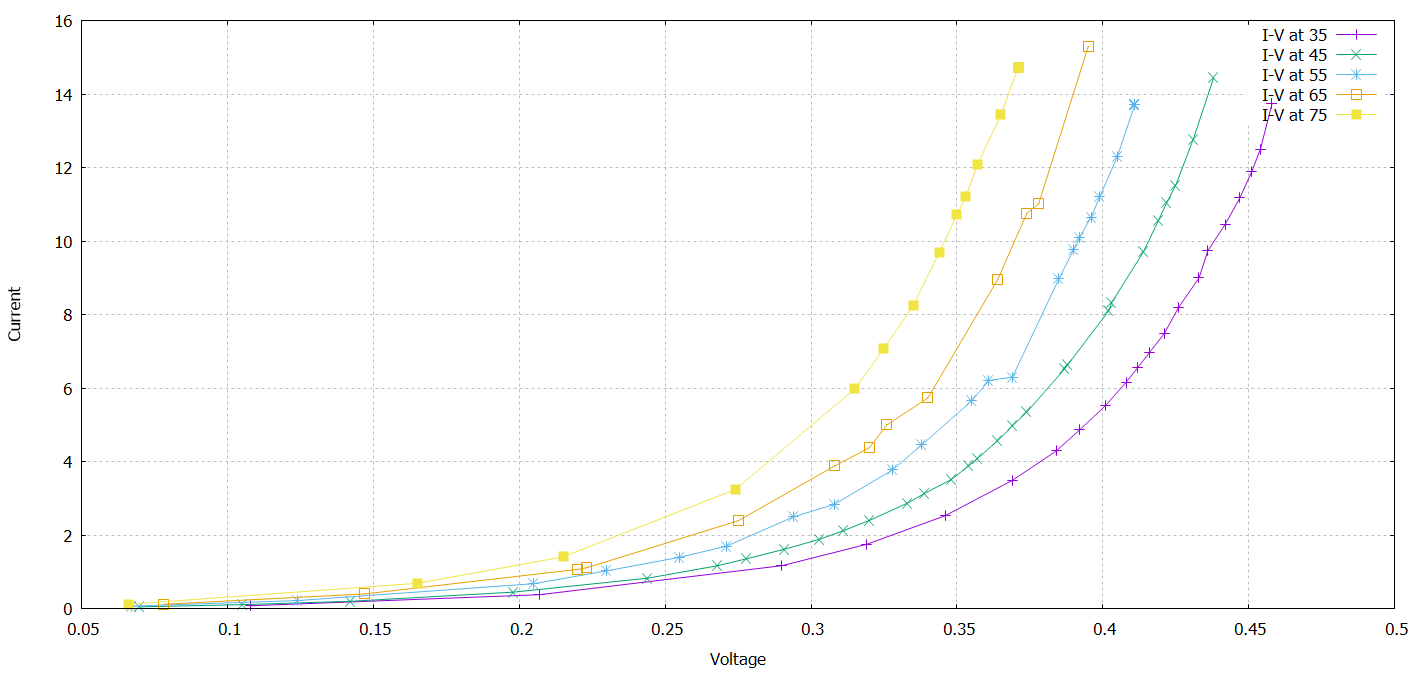
\includegraphics[width = \linewidth, trim = {0 0 0 0}, clip]{Part1_IV.png}
		\caption{I-V Characteristics}
	\end{subfigure}\\
	\begin{subfigure}[b]{\linewidth}
		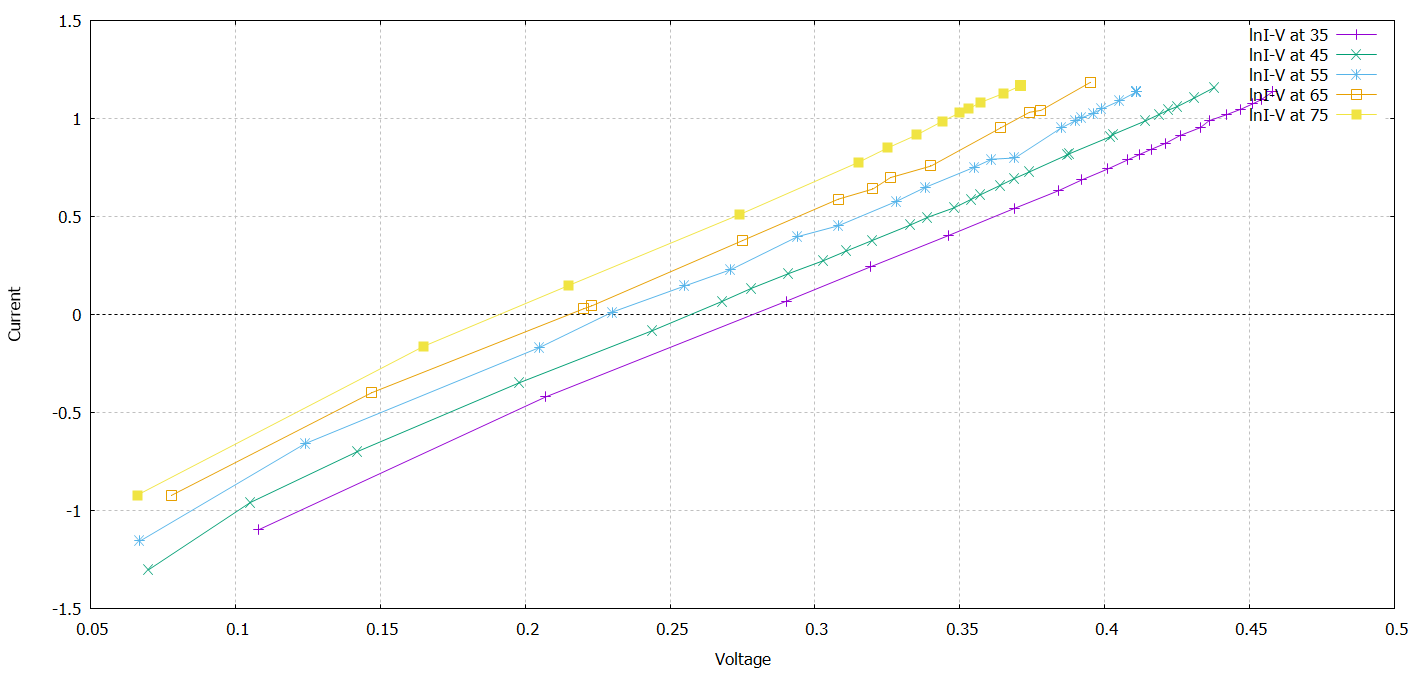
\includegraphics[width = \linewidth, trim = {0 0 0 0}, clip]{Part1_lnIV.png}
		\caption{ln(I)-V Characteristics}
	\end{subfigure} 
	\caption{Part 1}
\end{figure}

Now, using the values of \(I_D\) and \(ln(I_D)\) for a given \(V_D\), we can fill the observations table as follows:

\begin{center}
 \begin{tabular}{|| c | c | c | c | c | c ||} 
 \hline
 \hline
 Temp & \(V_D\), \(I_D = 1mA\) & \(V_D\), \(I_D = 2mA\) & \(V_D\), \(I_D = 5mA\) & \( \eta \), \(I_D = 1mA\) & \( \eta \), \( I_D = 5mA \) \\[0.25ex] 
 \hline\hline
 \(35^{\circ}C\) & 0.284 & 0.330 & 0.394 & 3.049 & 4.017 \\
 \(45^{\circ}C\) & 0.256 & 0.307 & 0.369 & 2.843 & 3.658 \\
 \(55^{\circ}C\) & 0.230 & 0.282 & 0.344 & 2.445 & 3.125 \\
 \(65^{\circ}C\) & 0.219 & 0.259 & 0.326 & 2.535 & 3.688 \\
 \(75^{\circ}C\) & 0.200 & 0.246 & 0.292 & 2.621 & 3.845 \\
 \hline 
\end{tabular}
\end{center}

\subsection{Part 2}

We obtained the readings of current flowing through the solar panel and voltage across the solar panel as mentioned in the table and plotted current vs voltage.
The plots are given below followed by the data values: 
\begin{figure}[H]
	\begin{subfigure}[b]{\linewidth}
	   	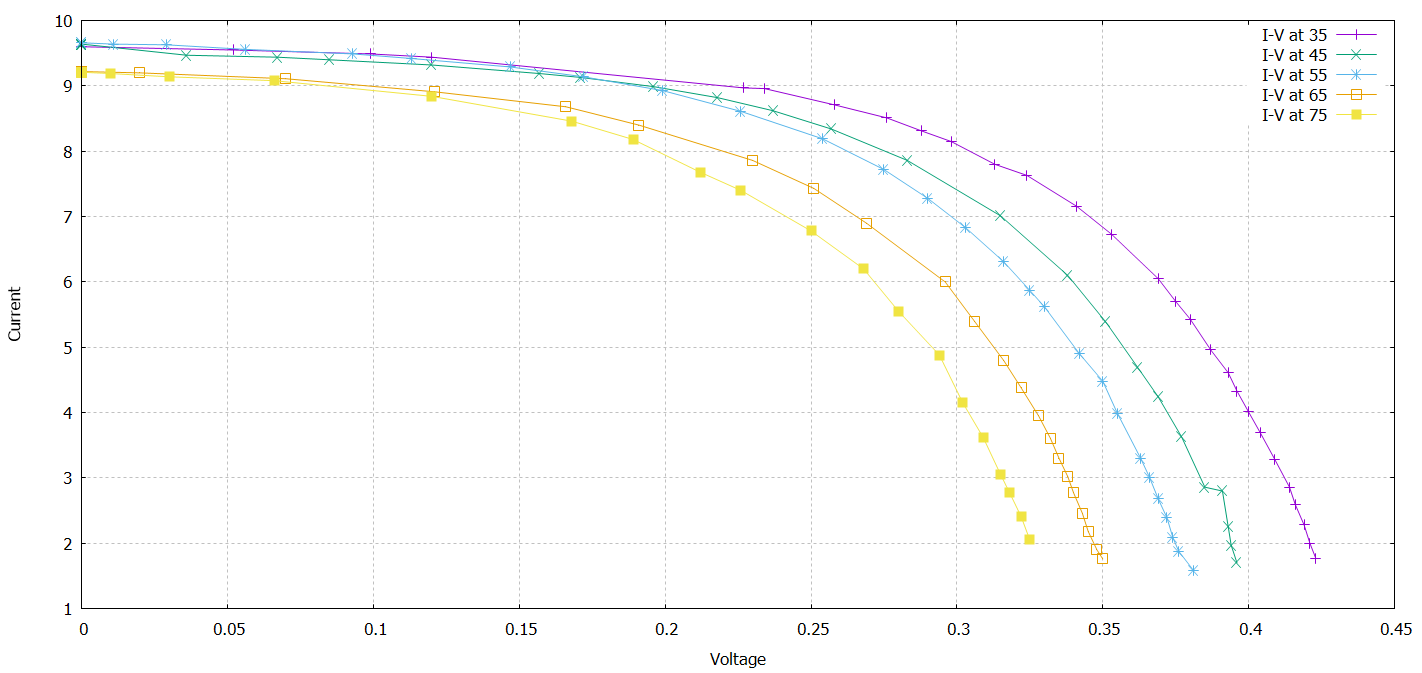
\includegraphics[width = 0.77\linewidth, trim = {0 0 0 0}, clip]{Part2_IV.png}
		\caption{I-V Characteristics}
	\end{subfigure}
	\begin{subfigure}[b]{\linewidth}
		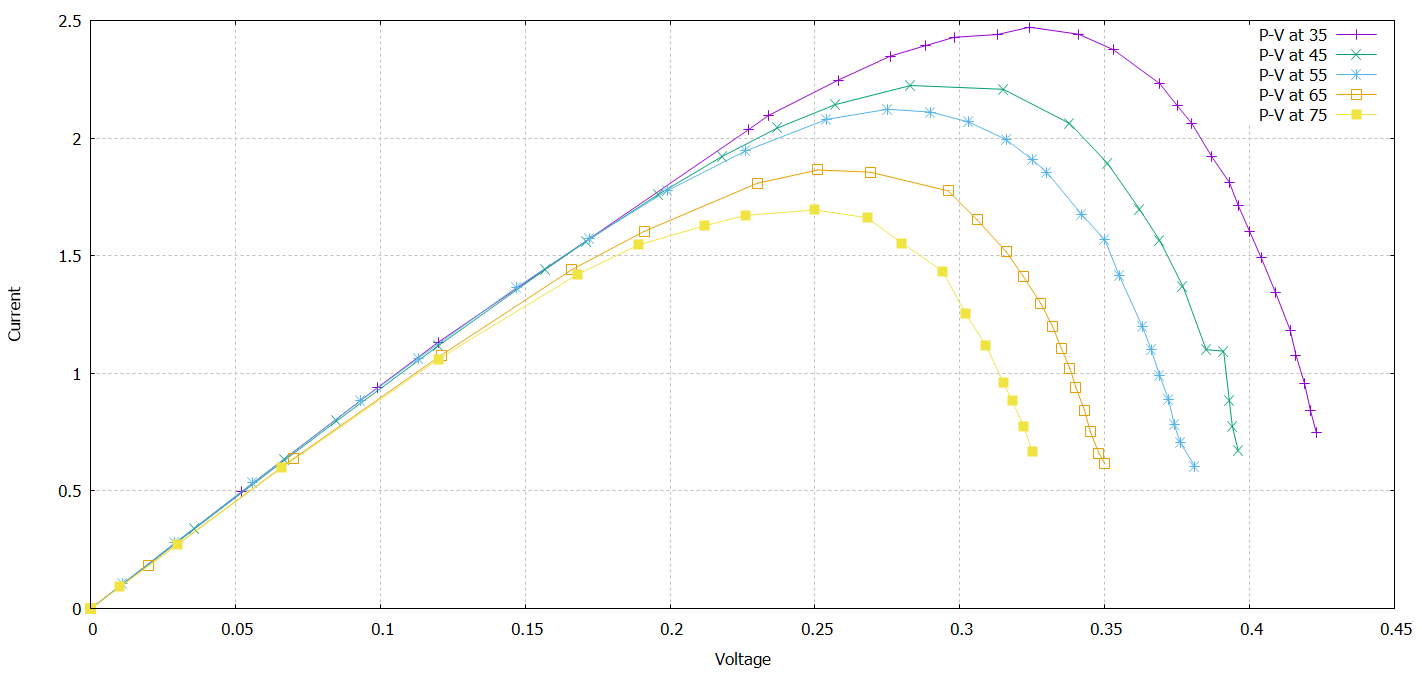
\includegraphics[width = 0.77\linewidth, trim = {0 0 0 0}, clip]{Part2_PV.png}
		\caption{P-V Characteristics}
	\end{subfigure} 
	\caption{Part 2}
\end{figure}

\begin{center}
 \begin{tabular}{|| c c | c c | c c | c c | c c ||} 
 \hline
 \multicolumn{2}{||c|}{\(35^{\circ}C\)} & \multicolumn{2}{c|}{\(45^{\circ}C\)} & \multicolumn{2}{c||}{\(55^{\circ}C\)} & \multicolumn{2}{c||}{\(65^{\circ}C\)} & \multicolumn{2}{c||}{\(75^{\circ}C\)}\\
 \hline
 \hline
 \( V_{SOL} \) & \( I_{SOL} \) & \( V_{SOL} \) & \( I_{SOL} \) & \( V_{SOL} \) & \( I_{SOL} \) & \( V_{SOL} \) & \( I_{SOL} \) & \( V_{SOL} \) & \( I_{SOL} \) \\ [0.25ex] 
 \hline\hline
 \hline 
0.423 & 1.77 & 0.396 & 1.7 & 0.381 & 1.59 & 0.35 & 1.76 & 0.325 & 2.05 \\ \hline 
0.421 & 2 & 0.394 & 1.97 & 0.376 & 1.88 & 0.348 & 1.9 & 0.322 & 2.41 \\ \hline 
0.419 & 2.28 & 0.393 & 2.25 & 0.374 & 2.09 & 0.345 & 2.18 & 0.318 & 2.78 \\ \hline 
0.416 & 2.59 & 0.391 & 2.8 & 0.372 & 2.39 & 0.343 & 2.46 & 0.315 & 3.05 \\ \hline 
0.414 & 2.86 & 0.385 & 2.86 & 0.369 & 2.68 & 0.34 & 2.77 & 0.309 & 3.62 \\ \hline 
0.409 & 3.28 & 0.377 & 3.63 & 0.366 & 3.01 & 0.338 & 3.02 & 0.302 & 4.15 \\ \hline 
0.404 & 3.69 & 0.369 & 4.24 & 0.363 & 3.3 & 0.335 & 3.3 & 0.294 & 4.88 \\ \hline 
0.4 & 4.01 & 0.362 & 4.69 & 0.355 & 3.99 & 0.332 & 3.61 & 0.28 & 5.55 \\ \hline 
0.396 & 4.33 & 0.351 & 5.39 & 0.35 & 4.48 & 0.328 & 3.95 & 0.268 & 6.2 \\ \hline 
0.393 & 4.61 & 0.338 & 6.1 & 0.342 & 4.9 & 0.322 & 4.38 & 0.25 & 6.78 \\ \hline 
0.387 & 4.96 & 0.315 & 7.01 & 0.33 & 5.62 & 0.316 & 4.8 & 0.226 & 7.4 \\ \hline 
0.38 & 5.43 & 0.283 & 7.86 & 0.325 & 5.87 & 0.306 & 5.4 & 0.212 & 7.68 \\ \hline 
0.375 & 5.7 & 0.257 & 8.34 & 0.316 & 6.31 & 0.296 & 6 & 0.189 & 8.18 \\ \hline 
0.369 & 6.05 & 0.237 & 8.62 & 0.303 & 6.83 & 0.269 & 6.9 & 0.168 & 8.46 \\ \hline 
0.353 & 6.73 & 0.218 & 8.82 & 0.29 & 7.28 & 0.251 & 7.43 & 0.12 & 8.84 \\ \hline 
0.341 & 7.16 & 0.196 & 8.99 & 0.275 & 7.72 & 0.23 & 7.86 & 0.066 & 9.08 \\ \hline 
0.324 & 7.63 & 0.171 & 9.13 & 0.254 & 8.19 & 0.191 & 8.4 & 0.03 & 9.14 \\ \hline 
0.313 & 7.8 & 0.157 & 9.19 & 0.226 & 8.61 & 0.166 & 8.68 & 0.01 & 9.19 \\ \hline 
0.298 & 8.15 & 0.12 & 9.32 & 0.199 & 8.93 & 0.121 & 8.91 & 0 & 9.21 \\ \hline 
0.288 & 8.31 & 0.085 & 9.4 & 0.172 & 9.14 & 0.07 & 9.11 & 0 & 9.21 \\ \hline 
0.276 & 8.51 & 0.067 & 9.44 & 0.147 & 9.29 & 0.02 & 9.2 & - & - \\ \hline 
0.258 & 8.71 & 0.036 & 9.47 & 0.113 & 9.42 & 0 & 9.22 & - & - \\ \hline 
0.234 & 8.96 & 0 & 9.64 & 0.093 & 9.49 & - & - & - & - \\ \hline 
0.227 & 8.97 & - & - & 0.056 & 9.56 & - & - & - & - \\ \hline 
0.12 & 9.44 & - & - & 0.029 & 9.63 & - & - & - & - \\ \hline 
0.099 & 9.49 & - & - & 0.011 & 9.64 & - & - & - & - \\ \hline 
0.052 & 9.55 & - & - & 0 & 9.66 & - & - & - & - \\ \hline 
0 & 9.6 & - & - & - & - & - & - & - & - \\ \hline 
\end{tabular}
\end{center}

The power for a given voltage at a given temperature can be calculated from this data:

\begin{center}
 \begin{tabular}{|| c c | c c | c c | c c | c c ||} 
 \hline
 \multicolumn{2}{||c|}{\(35^{\circ}C\)} & \multicolumn{2}{c|}{\(45^{\circ}C\)} & \multicolumn{2}{c||}{\(55^{\circ}C\)} & \multicolumn{2}{c||}{\(65^{\circ}C\)} & \multicolumn{2}{c||}{\(75^{\circ}C\)}\\
 \hline
 \hline
 \( V_{SOL} \) & \( P_{SOL} \) & \( V_{SOL} \) & \( P_{SOL} \) & \( V_{SOL} \) & \( P_{SOL} \) & \( V_{SOL} \) & \( P_{SOL} \) & \( V_{SOL} \) & \( P_{SOL} \) \\ [0.25ex] 
 \hline\hline
 \hline 
0.423 & 1.77 & 0.396 & 1.7 & 0.381 & 1.59 & 0.35 & 1.76 & 0.325 & 2.05 \\ \hline 
0.421 & 2 & 0.394 & 1.97 & 0.376 & 1.88 & 0.348 & 1.9 & 0.322 & 2.41 \\ \hline 
0.419 & 2.28 & 0.393 & 2.25 & 0.374 & 2.09 & 0.345 & 2.18 & 0.318 & 2.78 \\ \hline 
0.416 & 2.59 & 0.391 & 2.8 & 0.372 & 2.39 & 0.343 & 2.46 & 0.315 & 3.05 \\ \hline 
0.414 & 2.86 & 0.385 & 2.86 & 0.369 & 2.68 & 0.34 & 2.77 & 0.309 & 3.62 \\ \hline 
0.409 & 3.28 & 0.377 & 3.63 & 0.366 & 3.01 & 0.338 & 3.02 & 0.302 & 4.15 \\ \hline 
0.404 & 3.69 & 0.369 & 4.24 & 0.363 & 3.3 & 0.335 & 3.3 & 0.294 & 4.88 \\ \hline 
0.4 & 4.01 & 0.362 & 4.69 & 0.355 & 3.99 & 0.332 & 3.61 & 0.28 & 5.55 \\ \hline 
0.396 & 4.33 & 0.351 & 5.39 & 0.35 & 4.48 & 0.328 & 3.95 & 0.268 & 6.2 \\ \hline 
0.393 & 4.61 & 0.338 & 6.1 & 0.342 & 4.9 & 0.322 & 4.38 & 0.25 & 6.78 \\ \hline 
0.387 & 4.96 & 0.315 & 7.01 & 0.33 & 5.62 & 0.316 & 4.8 & 0.226 & 7.4 \\ \hline 
0.38 & 5.43 & 0.283 & 7.86 & 0.325 & 5.87 & 0.306 & 5.4 & 0.212 & 7.68 \\ \hline 
0.375 & 5.7 & 0.257 & 8.34 & 0.316 & 6.31 & 0.296 & 6 & 0.189 & 8.18 \\ \hline 
0.369 & 6.05 & 0.237 & 8.62 & 0.303 & 6.83 & 0.269 & 6.9 & 0.168 & 8.46 \\ \hline 
0.353 & 6.73 & 0.218 & 8.82 & 0.29 & 7.28 & 0.251 & 7.43 & 0.12 & 8.84 \\ \hline 
0.341 & 7.16 & 0.196 & 8.99 & 0.275 & 7.72 & 0.23 & 7.86 & 0.066 & 9.08 \\ \hline 
0.324 & 7.63 & 0.171 & 9.13 & 0.254 & 8.19 & 0.191 & 8.4 & 0.03 & 9.14 \\ \hline 
0.313 & 7.8 & 0.157 & 9.19 & 0.226 & 8.61 & 0.166 & 8.68 & 0.01 & 9.19 \\ \hline 
0.298 & 8.15 & 0.12 & 9.32 & 0.199 & 8.93 & 0.121 & 8.91 & 0 & 9.21 \\ \hline 
0.288 & 8.31 & 0.085 & 9.4 & 0.172 & 9.14 & 0.07 & 9.11 & 0 & 9.21 \\ \hline 
0.276 & 8.51 & 0.067 & 9.44 & 0.147 & 9.29 & 0.02 & 9.2 & - & - \\ \hline 
0.258 & 8.71 & 0.036 & 9.47 & 0.113 & 9.42 & 0 & 9.22 & - & - \\ \hline 
0.234 & 8.96 & 0 & 9.64 & 0.093 & 9.49 & - & - & - & - \\ \hline 
0.227 & 8.97 & - & - & 0.056 & 9.56 & - & - & - & - \\ \hline 
0.12 & 9.44 & - & - & 0.029 & 9.63 & - & - & - & - \\ \hline 
0.099 & 9.49 & - & - & 0.011 & 9.64 & - & - & - & - \\ \hline 
0.052 & 9.55 & - & - & 0 & 9.66 & - & - & - & - \\ \hline 
0 & 9.6 & - & - & - & - & - & - & - & - \\ \hline 
\end{tabular}
\end{center}

Hence, we can calculate the open circuit voltage, short circuit current, maximum power and fill factor from the given data:

\begin{center}
 \begin{tabular}{|| c | c | c | c | c |c ||} 
 \hline
 \hline
 Temp & \(V_{OC}\) & \(I_{SC}\) & \(V_{MP}\) & \(I_{MP}\) & FF \\[0.25ex] 
 \hline\hline
 \(35^{\circ}C\) & 0.436 & 9.60 & 0.324 & 7.63 & 0.591 \\ 
 \(45^{\circ}C\) & 0.408 & 9.64 & 0.283 & 7.86 & 0.566 \\ 
 \(55^{\circ}C\) & 0.393 & 9.66 & 0.275 & 7.72 & 0.559 \\ 
 \(65^{\circ}C\) & 0.365 & 9.22 & 0.251 & 7.43 & 0.554 \\ 
 \(75^{\circ}C\) & 0.342 & 9.21 & 0.250 & 6.78 & 0.538 \\ 
 \hline 

\end{tabular}
\end{center}

\section{Simulation}
\begin{enumerate}
\item \textbf{Part 1}

\begin{verbatim}
Solar Cell I-V Characteristics

.include Solar_Cell.txt

x1 1 0 solar_cell
vin 2 0 dc 1 ac 0
r1 2 1 100

.dc vin -2 2 0.01

.control
run

plot ((v(2)-v(1))/100) vs v(1)

.endc
.end
\end{verbatim}


\item \textbf{Part 2}

\begin{verbatim}
Solar Cell I-V Characteristics

.include Solar_Cell.txt

x1 1 0 solar_cell
r1 2 0 1
v1 1 2 0

.dc r1 1 500 0.05

.control
run

plot i(v1) vs v(1)

.endc
.end
\end{verbatim}

\item \textbf{Solar Cell}

\begin{verbatim}
* Solar Cell SPICE Subcircuit Data

.subckt solar_cell PX NX

*IL is photo generated current
*IL NX TMP dc 0e-3
*IL NX TMP dc 8e-3
IL NX TMP dc 10e-3

.temp 35

d1 TMP NX diode
.model diode d (is=(1e-13) n=1)

d2 TMP NX diode2
.model diode2 d (is=(2e-6) n=2)

*rs TMP PX 0
rs TMP PX 10
*rs TMP PX 30

*rsh TMP NX 5e2
*rsh TMP NX 1e3
rsh TMP NX 5e3

.ends solar_cell

*Developed by Wadhwani Electronics Lab
*Dept. of Electrical Engg.
*IIT Bombay
*January 09, 2015.
\end{verbatim}
\end{enumerate}

For part 1, based on the simulation, here is the observation table mentioning \(V_D\) and \(\eta\) for different values of \(I_D\):

\begin{center}
 \begin{tabular}{|| c | c | c | c | c | c ||} 
 \hline
 \hline
 Temp & \(V_D\), \(I_D = 1mA\) & \(V_D\), \(I_D = 2mA\) & \(V_D\), \(I_D = 5mA\) & \( \eta \), \(I_D = 1mA\) & \( \eta \), \( I_D = 5mA \) \\[0.25ex] 
 \hline\hline
 \(35^{\circ}C\) & 0.3072 & 0.3525 & 0.4342 & 2.6079 & 4.1327 \\
 \(45^{\circ}C\) & 0.2781 & 0.3270 & 0.4075 & 2.5699 & 4.0538 \\
 \(55^{\circ}C\) & 0.2491 & 0.2960 & 0.3806 & 2.5256 & 3.9780 \\
 \(65^{\circ}C\) & 0.2202 & 0.2707 & 0.3538 & 2.4700 & 3.9042 \\
 \(75^{\circ}C\) & 0.1956 & 0.2426 & 0.3288 & 2.4206 & 3.8592 \\
 \hline 

\end{tabular}
\end{center}

\begin{figure}[H]
	\begin{subfigure}[b]{0.6\linewidth}
	   	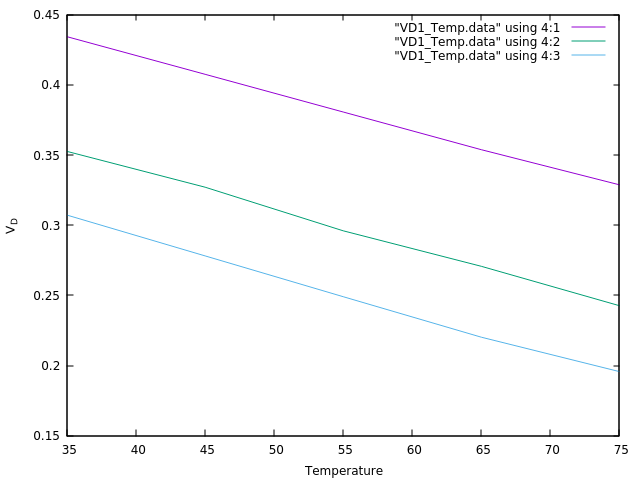
\includegraphics[width = \linewidth, trim = {0 0 0 0}, clip]{Pt1_VDTemp.png}
		\caption{\( V_D \) vs Temp }
	\end{subfigure}
	\begin{subfigure}[b]{0.6\linewidth}
		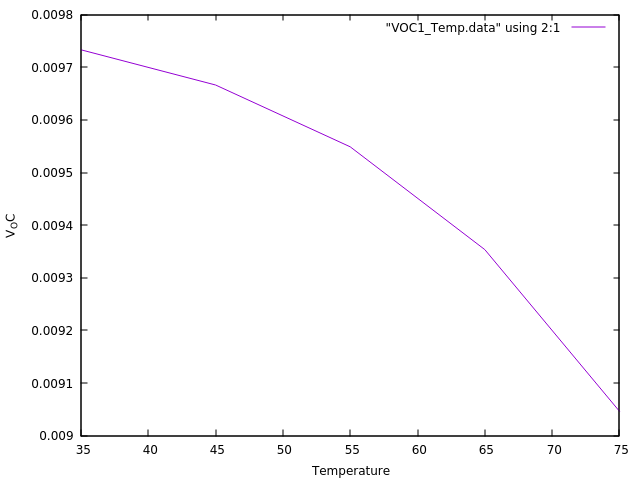
\includegraphics[width = \linewidth, trim = {0 0 0 0}, clip]{Pt1_VOCTemp.png}
		\caption{\( V_{OC} \) vs Temp}
	\end{subfigure} 
	\caption{Part 1}
\end{figure}

For the lighted solar cell simulation, here are the plotted results:

\begin{figure}[H]
	\begin{subfigure}[b]{0.6\linewidth}
	   	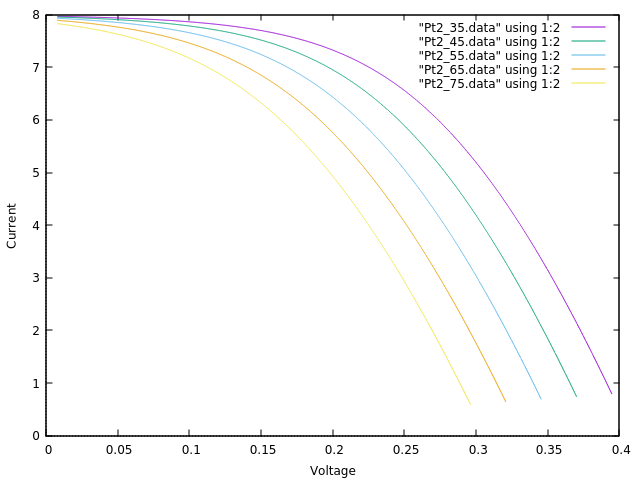
\includegraphics[width = \linewidth, trim = {0 0 0 0}, clip]{Pt2_IV.png}
		\caption{I-V Characteristics}
	\end{subfigure}
	\begin{subfigure}[b]{0.6\linewidth}
		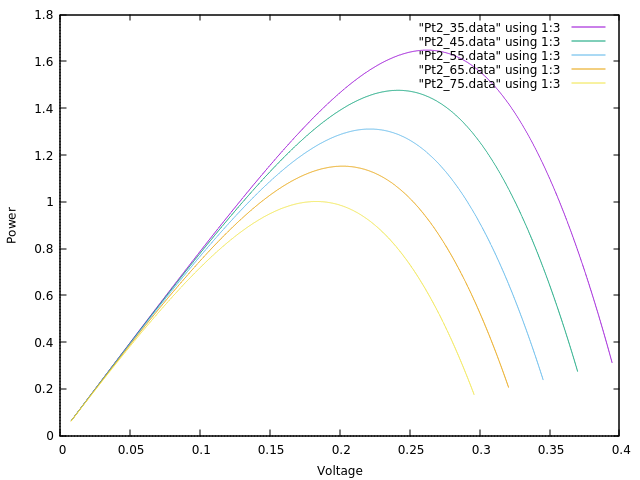
\includegraphics[width = \linewidth, trim = {0 0 0 0}, clip]{Pt2_PV.png}
		\caption{P-V Characteristics}
	\end{subfigure} 
	\begin{subfigure}[b]{0.6\linewidth}
	   	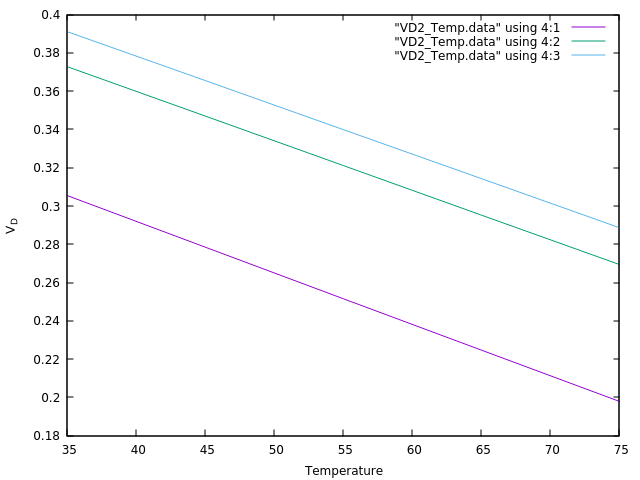
\includegraphics[width = \linewidth, trim = {0 0 0 0}, clip]{Pt2_VDTemp.png}
		\caption{\( V_D \) vs Temp}
	\end{subfigure}
	\begin{subfigure}[b]{0.6\linewidth}
		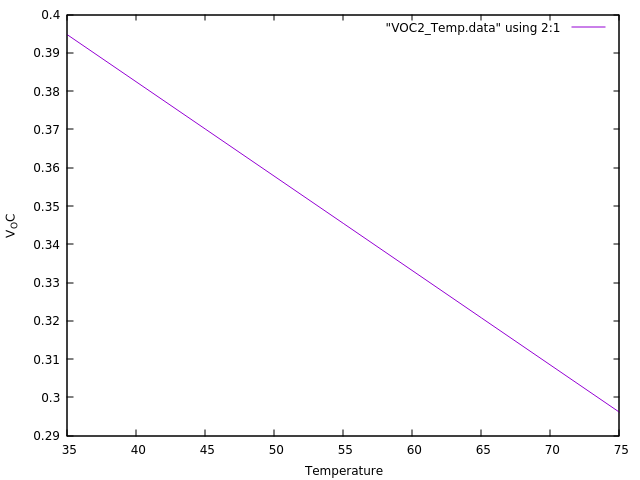
\includegraphics[width = \linewidth, trim = {0 0 0 0}, clip]{Pt2_VOCTemp.png}
		\caption{\( V_{OC} \) vs Temp}
	\end{subfigure} 
	\begin{subfigure}[b]{0.6\linewidth}
	   	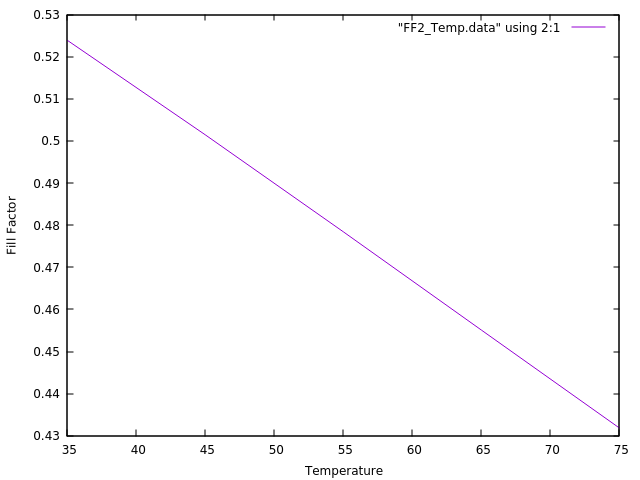
\includegraphics[width = \linewidth, trim = {0 0 0 0}, clip]{Pt2_FFTemp.png}
		\caption{Fill Factor vs Temp}
	\end{subfigure}
	\caption{Part 2}
\end{figure}

For the third figure for part 2 giving \( V_D \) vs Temperature, the purple line represents \( I_D = 5mA \), the green line represents \( I_D = 2mA \) and the blue line represents \( I_D = 1mA \).\\

From the values given in part 2, we can calculate the values of open circuit voltages, short circuit currents, maximum power voltage, maximum power current and fill factors for the given five temperatures:
\begin{center}
 \begin{tabular}{|| c | c | c | c | c |c ||} 
 \hline
 \hline
 Temp & \(V_{OC}\) & \(I_{SC}\) & \(V_{MP}\) & \(I_{MP}\) & FF \\[0.25ex] 
 \hline\hline
 \(35^{\circ}C\) & 0.3948 & 7.9672 & 0.2625 & 6.2791 & 0.5239 \\
 \(45^{\circ}C\) & 0.3702 & 7.9536 & 0.2418 & 6.1059 & 0.5015 \\
 \(55^{\circ}C\) & 0.3455 & 7.9301 & 0.2217 & 5.9122 & 0.4784 \\
 \(65^{\circ}C\) & 0.3208 & 7.8911 & 0.2021 & 5.7007 & 0.4551 \\
 \(75^{\circ}C\) & 0.2961 & 7.8287 & 0.1833 & 5.4626 & 0.4318 \\
 \hline 

\end{tabular}
\end{center}

\section{Inference}

\subsection{Part 1}

In order to explain the trends we see, we bring in the solar cell equation when it is kept in the dark:
\[ I = I_{01}\left[ e^{\frac{qV_D}{kT}} - 1\right] + I_{02}\left[ e^{\frac{qV_D}{2kT}} - 1\right] + \frac{V-IR_s}{R_{SH}}\]
Ideality factor decreases with increase in temperature. The inverse proportionality of the ideality factor with respect to temperature is expected as the term of higher ideality factor has a higher effect at a lower temperature. At higher temperatures, the term of higher ideality factor dies faster than the term of lower ideality factor.\\\\
Ideality factor decreases with an increase in current. This is explained by the opposite reason. An increase in current is implied by the increase in voltage. As voltage increases, the term with higher ideality factor tends to increase faster than the term with lower ideality factor. Hence the ideality factor of the solar cell increases as a whole.\\
Apart from this, there is a significant effect of \( R_s \) and \( R_{SH} \), due to parasitic losses and manufacturing effects. These may also have an effect in the overall ideality factor which is calculated from the slope of the ln(I)-V characteristics.\\\\
For a given voltage, the current flowing through the diode increases with temperature. We know that the resistance of a normal semiconductor decreases with temperature. Since the quasi-neutral regions behave as semiconductors, this inverse proportionality of resistance with respect to temperature can be brought forward as the reason of the increase of current at a given voltage. Equivalently, we can say that for a given current, voltage decreases with an increase in temperature. This is quite visible when we tabulate \( V_D \) for a fixed \( I_D \) varying temperature.

\subsection{Part 2}

In order to explain the trends we see, we bring in the solar cell equation when it is kept lighted:
\[ I = I_{01}\left[ e^{\frac{qV_D}{kT}} - 1\right] + I_{02}\left[ e^{\frac{qV_D}{2kT}} - 1\right] + \frac{V-IR_s}{R_{SH}} - I_L\]
Open circuit voltage is a value which depends on the width of the depletion region. Since we know that the width of the depletion region shares an inverse relationship with temperature, the open circuit voltage decreases with temperature.\\\\
A similar argument can be said about the short circuit current. However the rate of decrease of the short circuit current is smaller than that of open circuit voltage. This statement can be justified by the same reason as that for the increase in current at a given voltage when the solar cell is kept in the dark, which is that the resistance of the quasi-neutral regions reduces with temperature. This has an increasing effect on current.\\\\
An equivalent and higher rate of decrease occurs in the case of the voltage at the maximum power point (MPP), \( V_{MP} \) and the current at the maximum power point (MPP), \( I_{MP} \). This higher rate of decrease is what causes the eventual decrease in the fill factor with respect to temperature; i.e. the temperature coefficient of fill factor is negative.

\end{document}
